\chapter{Цветовые представления, адроны и конфайнмент}

\paragraph{Короткое вступительное отступление.}
Прежде чем вернуться к теории групп, позвольте одну бесстыдную рекламу. \emph{The Black Hole War} рассказывает историю долгого спора со Стивеном Хокингом о том, уничтожают ли черные дыры квантовую информацию. В ней также зафиксирована некоторая жестокость, свойственная теоретическим физикам: не только кот Шрёдингера, но и рыбки Сасскинда с их прискорбным путешествием в унитаз. Исполнив этот долг, вернемся к Алисе и Бобу. Алиса по-прежнему страдает, потому что Боб по-прежнему заставляет ее учить теорию групп.

\lectureoverview{Симметрия становится физической благодаря своему действию на состояния. Мы начнем с вращений, чтобы ввести представления и генераторы, а затем повторим это построение для цветовой группы \(SU(3)\). Цветовые представления объединяются в адроны, а их динамика объясняет, почему изолированный цвет никогда не наблюдается.}

\section{Группа и объекты, на которые она действует}

В любом обсуждении симметрии присутствуют две идеи. Во-первых, есть абстрактная группа: совокупность операций с законом умножения, единичным элементом и обратными элементами. Во-вторых, есть объекты, на которые эти операции действуют. Эти две идеи можно различать, но в физике их нельзя разделить. Симметрия важна потому, что она преобразует физические состояния, поля, координаты или наблюдаемые.

\begin{classroomqa}
\audiencequestion{Группа была описана и как абстрактная таблица умножения, и как матрицы, действующие на физические объекты. Можно ли отделить эти две части друг от друга?\lecturetimestamp{00:01:58}}
\lecturerresponse{Это разные уровни описания, но они полностью взаимосвязаны. Вращение существует как абстрактная операция еще до того, как мы укажем, что именно оно вращает. Затем физика спрашивает, как эта же операция действует на состояния и величины, относящиеся к данной системе. Матрицы задают это конкретное действие, сохраняя при этом абстрактный закон умножения.}
\end{classroomqa}

Пространственные вращения дают самый наглядный пример. Классически одно и то же вращение может действовать на координаты частицы, на направление магнита или на любой другой вектор. В квантовой механике состояния живут в линейном векторном пространстве, поэтому вращение представляется линейным оператором в этом пространстве. Если \(g\) обозначает абстрактный элемент группы, а \(D(g)\) — его матричный представитель, то согласованность означает
\begin{equation}
D(g_1g_2)=D(g_1)D(g_2),
\qquad
D(e)=\boldsymbol 1.
\end{equation}
Матрицы не обязаны быть похожи на абстрактные операции, но их умножение должно воспроизводить групповое умножение.
\editorialnote{Уравнение гомоморфизма явно записывает соответствие между групповым умножением и умножением матриц, которое в исходном тексте описано словами.}

Размерность матрицы определяется пространством состояний, а не одной только абстрактной группой. Если мы оставляем только спин одного электрона, то существуют две ортогональные возможности — спин вверх и спин вниз, — и состояние представляет собой двухкомпонентный столбец. Поэтому вращения действуют через матрицы \(2\times2\). Для двух объектов со спином 1/2 существуют четыре базисных состояния,
\begin{equation}
\ket{\uparrow\uparrow},\qquad
\ket{\uparrow\downarrow},\qquad
\ket{\downarrow\uparrow},\qquad
\ket{\downarrow\downarrow},
\end{equation}
и соответствующее действие на объединенном пространстве четырехмерно.

Хорошо знакомая последовательность такова
\begin{equation}
\begin{array}{c|c|c}
\text{spin} & \text{number of states} & \text{matrix dimension}\\
\hline
0 & 1 & 1\times1\\
\frac12 & 2 & 2\times2\\
1 & 3 & 3\times3\\
\frac32 & 4 & 4\times4
\end{array}
\end{equation}
и так далее. Состояние со спином нуль реализует тривиальное представление: любое вращение оставляет его неизменным. Матрица размерности один на один — это просто \(1\). Состояние со спином 1 имеет три компоненты, и его матрицы вращения — это обычные трехмерные векторные вращения. В более общем случае спин \(j\) имеет \(2j+1\) состояний.

Представление может быть и бесконечномерным. Если мы описываем полное орбитальное движение электрона, а не только его спин, то состояние содержит амплитуду для каждого положения или, эквивалентно, для каждого импульса. Тогда оператор вращения действует на бесконечномерном пространстве волновых функций. Таким образом, одна и та же абстрактная группа вращений имеет тривиальные, двумерные, трехмерные и бесконечномерные представления. Именно этот факт мы снова используем, когда обсуждение перейдет от спина к цвету.

\section{Почему спиновые вращения являются специальными унитарными преобразованиями}

Теперь вернемся к спину одного электрона и отбросим его орбитальное движение. Вращение представляется унитарной матрицей \(U\) размера \(2\times2\),
\begin{equation}
U^\dagger U=\boldsymbol 1,
\qquad
U^{-1}=U^\dagger.
\label{eq:l4-unitarity}
\end{equation}
Обратное преобразование должно отменять вращение, а унитарность сохраняет норму и, следовательно, любую вероятность.

Общая комплексная матрица размера \(2\times2\) содержит четыре комплексных элемента, то есть 8 вещественных параметров. Уравнение~\eqref{eq:l4-unitarity} накладывает 4 независимых вещественных условия, оставляя 4 параметра. Обычное пространственное вращение имеет только 3: два параметра задают ось и один задает угол. Поэтому унитарная матрица содержит одну лишнюю фазу. Дополнительное ограничение имеет вид
\begin{equation}
\det U=1.
\label{eq:l4-det-one}
\end{equation}
Тогда подсчет дает
\begin{equation}
8-4-1=3.
\end{equation}

Ограничение на единичный детерминант устойчиво относительно умножения, поскольку
\begin{equation}
\det(AB)=\det A\,\det B.
\end{equation}
Если каждая из двух матриц имеет детерминант 1, то то же верно и для их произведения. Оно также совместимо с унитарностью. Взяв детерминант от уравнения~\eqref{eq:l4-unitarity}, получаем
\begin{equation}
1=\det(U^\dagger U)
=\det(U^\dagger)\det U
=(\det U)^*\det U.
\end{equation}
Следовательно, детерминант унитарной матрицы лежит на единичной окружности,
\begin{equation}
\det U=e^{i\phi}.
\end{equation}

\begin{classroomqa}
\audiencequestion{Требует ли унитарность, чтобы детерминант был вещественным?\lecturetimestamp{00:12:10}}
\lecturerresponse{Нет. Унитарность требует только единичного модуля. Детерминант может быть любой чистой фазой \(e^{i\phi}\). Для двумерной матрицы умножение \(U\) на \(e^{-i\phi/2}\) устраняет эту общую фазу и дает матрицу с детерминантом 1.}
\end{classroomqa}

Действительно, если
\begin{equation}
V=e^{-i\phi/2}U,
\end{equation}
то \(V\) остается унитарной, и
\begin{equation}
\det V=e^{-i\phi}\det U=1.
\end{equation}
Унитарные матрицы с детерминантом 1 образуют \(SU(2)\).

Здесь есть одна тонкость. Возникает соблазн сказать, что \(SU(2)\) — это просто группа вращений в трехмерном пространстве, но соответствие здесь два к одному. Матрицы \(U\) и \(-U\) по-разному действуют на спинор, однако соответствуют одному и тому же вращению обычного вектора. Таким образом,
\begin{equation}
SU(2)/\{\boldsymbol 1,-\boldsymbol 1\}\simeq SO(3).
\end{equation}
Для настоящего обсуждения важны локальная структура умножения и три генератора, но двулистное накрытие объясняет двузначность вращений спина 1/2.

\section{Бесконечно малые преобразования и их генераторы}

Конечное вращение можно составить из множества очень малых вращений. Элемент группы, близкий к единичному, называется бесконечно малым, и знания всех бесконечно малых направлений достаточно, чтобы в связной группе восстановить конечные преобразования повторным умножением. Еще важнее для физики то, что операторы, порождающие эти бесконечно малые преобразования, являются сохраняющимися величинами, связанными с этой симметрией.

Запишем элемент, близкий к единице, в виде
\begin{equation}
U=\boldsymbol 1+i\epsilon T,
\qquad |\epsilon|\ll1.
\label{eq:l4-infinitesimal-u}
\end{equation}
Множитель \(i\) — удобное соглашение. Подстановка в условие унитарности и отбрасывание членов порядка \(\epsilon^2\) дает
\begin{align}
(\boldsymbol 1+i\epsilon T)
(\boldsymbol 1-i\epsilon T^\dagger)&=\boldsymbol 1,
\\
i\epsilon(T-T^\dagger)&=0,
\\
T&=T^\dagger.
\label{eq:l4-hermitian-generator}
\end{align}
Генератор эрмитов, как и должно быть для квантовомеханической наблюдаемой.

\begin{figure}[htbp]
\centering
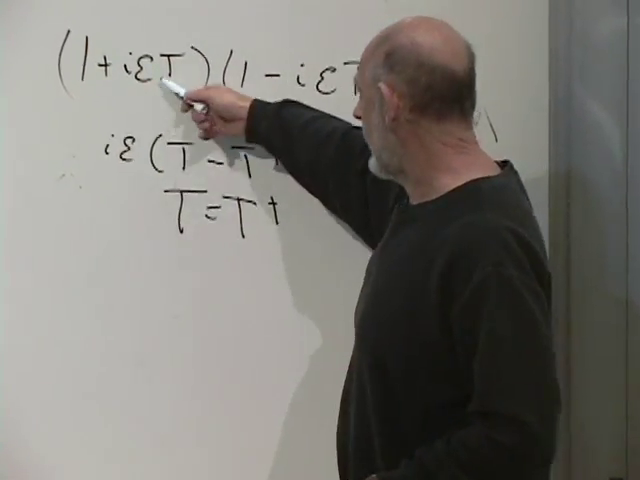
\includegraphics[width=0.62\textwidth]{lecture_04_figure_03.png}
\caption{Вычисление унитарности для элемента, близкого к единице, приводящее к \(T=T^\dagger\).}
\lectureframe{00:23:28}
\end{figure}

Для пространственных вращений существуют три линейно независимых генератора, потому что имеются три независимые бесконечно малые оси вращения. Малое вращение вокруг произвольной оси составляется из малых вращений вокруг \(x\), \(y\) и \(z\). Соответствующие генераторы — это операторы момента импульса \(J_x,J_y,J_z\). Их коммутаторы кодируют некоммутативность вращений,
\begin{equation}
[J_i,J_j]=i\epsilon_{ijk}J_k.
\label{eq:l4-angular-momentum-algebra}
\end{equation}
и из повторных бесконечно малых вращений затем строится конечное вращение.

Мы использовали унитарность, но еще не использовали условие единичного детерминанта. Для любой малой матрицы \(m\),
\begin{equation}
\det(\boldsymbol 1+\epsilon m)
=1+\epsilon\,\operatorname{tr}m+O(\epsilon^2).
\label{eq:l4-det-expansion}
\end{equation}

\begin{figure}[htbp]
\centering
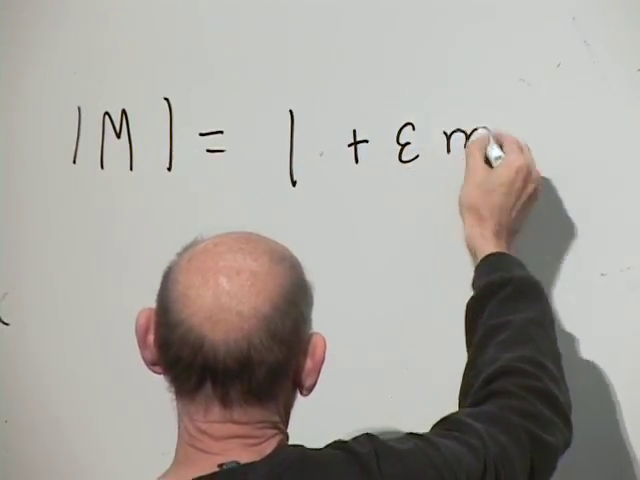
\includegraphics[width=0.62\textwidth]{lecture_04_figure_02.png}
\caption{Разложение детерминанта по первому порядку в том виде, в каком оно начинается на доске.}
\lectureframe{00:21:51}
\end{figure}

Применяя уравнение~\eqref{eq:l4-det-expansion} к уравнению~\eqref{eq:l4-infinitesimal-u},
\begin{equation}
\det U
=1+i\epsilon\,\operatorname{tr}T+O(\epsilon^2).
\end{equation}
Следовательно, условие специальной унитарности требует
\begin{equation}
\operatorname{tr}T=0.
\label{eq:l4-traceless-generator}
\end{equation}
Генераторы \(SU(2)\) — это в точности бесследовые эрмитовы матрицы \(2\times2\). Это векторное пространство имеет размерность 3. Стандартный базис задается матрицами Паули,
\begin{equation}
\begin{aligned}
\sigma_x&=
\begin{pmatrix}0&1\\1&0\end{pmatrix},
&
\sigma_y&=
\begin{pmatrix}0&-i\\i&0\end{pmatrix},
\\[0.4em]
\sigma_z&=
\begin{pmatrix}1&0\\0&-1\end{pmatrix}.
\end{aligned}
\end{equation}
Для представления со спином 1/2 можно взять \(J_i=\sigma_i/2\), так что конечное вращение на угол \(\theta\) вокруг \(\hat{\boldsymbol n}\) имеет вид
\begin{equation}
U(\hat{\boldsymbol n},\theta)
=\exp\!\left(-i\theta\,
\hat{\boldsymbol n}\cdot\boldsymbol\sigma/2\right).
\end{equation}
\editorialnote{Конечная экспонента является стандартным завершением обсуждения бесконечно малых генераторов. В исходном тексте подчеркиваются повторные малые вращения, а не явная запись этой формулы.}

\begin{classroomqa}
\audiencequestion{Итак, существуют три независимые бесследовые эрмитовы матрицы \(2\times2\)?\lecturetimestamp{00:24:07}}
\lecturerresponse{Да. Это три матрицы Паули. Для специальных унитарных матриц \(3\times3\) соответствующее число равно 8, и стандартный базис задается восемью матрицами Гелл-Манна.}
\end{classroomqa}

\begin{classroomqa}
\audiencequestion{Это та самая ``восьмёрка'', что и в восьмеричном пути и у восьми глюонов?
\lecturetimestamp{00:24:43}}
\lecturerresponse{Математика здесь — один и тот же тип теории представлений \(SU(3)\), но нужно указать, какая именно симметрия \(SU(3)\) действует. Историческая вкусовая симметрия восьмеричного пути — не цветовая \(SU(3)\). Восемь глюонов принадлежат присоединённому представлению цветовой \(SU(3)\).}
\end{classroomqa}

\section{От SU(2) к цветовой SU(3)}

Теперь увеличим матрицы с \(2\times2\) до \(3\times3\). Общая комплексная
\(3\times3\)-матрица имеет девять комплексных элементов, а значит, 18 вещественных параметров.
Условие \(U^\dagger U=\boldsymbol 1\) даёт 9 вещественных ограничений,
а \(\det U=1\) устраняет ещё одно. Поэтому
\begin{equation}
18-9-1=8.
\end{equation}
Имеются 8 независимых бесконечно малых направлений и 8 бесследовых
эрмитовых генераторов. В отличие от \(SU(2)\), эта группа не является группой вращений
обычного трёхмерного пространства. Это внутренняя симметрия, действующая на
цвет.

Прежде чем приписывать эти представления кваркам, вспомним, как возникают составные
представления. Соединим две системы со спином одна вторая и пренебрежём
их орбитальным движением. Получаются 4 состояния произведения, но вращение не перемешивает все 4 в одно неприводимое представление. Три комбинации преобразуются как спин 1,
\begin{align}
\ket{1,1}&=\ket{\uparrow\uparrow},\\
\ket{1,0}&=\frac{1}{\sqrt2}
(\ket{\uparrow\downarrow}+\ket{\downarrow\uparrow}),\\
\ket{1,-1}&=\ket{\downarrow\downarrow},
\end{align}
тогда как четвёртая преобразуется как спин 0,
\begin{equation}
\ket{0,0}=\frac{1}{\sqrt2}
(\ket{\uparrow\downarrow}-\ket{\downarrow\uparrow}).
\end{equation}
Следовательно,
\begin{equation}
\boldsymbol 2\otimes\boldsymbol 2
=\boldsymbol 3\oplus\boldsymbol 1.
\label{eq:l4-two-spin-decomposition}
\end{equation}
Состояния с сонаправленными спинами дают члены триплета с \(m=\pm1\), симметричное
состояние с нулевой проекцией завершает его, а антисимметричная комбинация является
синглетом. Именно такова общая логика сложения угловых моментов и объединения
цветовых представлений.

То же различие синглет--триплет возникает всякий раз, когда связываются две степени свободы
со спином одна вторая. В атомарном водороде спины электрона и протона
образуют сверхтонкие синглетное и триплетное состояния. В орто- и параводороде
та же теория представлений описывает ядерные спины двух протонов в молекуле
\(H_2\).
\editorialnote{В исходном тексте выражение ``орто- и параводород'' употребляется при обсуждении спинов в системе протон--электрон в атоме водорода. Математическое разложение верно; для точности здесь различаются молекулярные и атомные названия.}

\subsection{Триплет и антитриплет}

У отдельного кварка есть три цветовые амплитуды. В выбранном базисе запишем
\begin{equation}
q=
\begin{pmatrix}
q_r\\q_g\\q_b
\end{pmatrix},
\qquad
q'=Uq,
\qquad U\in SU(3).
\label{eq:l4-quark-triplet}
\end{equation}
Эти три компоненты могут быть амплитудами состояния одного кварка или тремя
операторами поля, создающими красный, зелёный и синий кварки. Группа перемешивает
три компоненты. Состояние, которое первоначально было красным, после цветового преобразования
вообще говоря становится суперпозицией красного, зелёного и синего. Это фундаментальное
трёхмерное представление называется \(\boldsymbol 3\).

Для антикварка группа действует через комплексно-сопряжённое к кварковому
представление. Взяв комплексное сопряжение уравнения~\eqref{eq:l4-quark-triplet}, получаем
\begin{equation}
\bar q'=U^*\bar q.
\end{equation}
Это представление обозначается \(\bar{\boldsymbol 3}\). Аналогия с \(U(1)\)
непосредственна: если электронное поле приобретает \(e^{i\theta}\), то позитронное поле
приобретает \(e^{-i\theta}\). Цветовые преобразования кварка и антикварка —
неабелева версия такого сопряжённого соответствия.

В окрестности единицы, если
\begin{equation}
U=\boldsymbol 1+i\epsilon T,
\end{equation}
то
\begin{equation}
U^*=\boldsymbol 1-i\epsilon T^*.
\end{equation}
Следовательно, генераторы антитриплета равны \(-T^*\), то есть это сопряжённые генераторы с противоположным
знаком. Именно в этом точном смысле антикварки несут противоположные цветовые
заряды.

\begin{classroomqa}
\audiencequestion{Что происходит с комплексно-сопряжённым представлением в случае \(SU(2)\)?
\lecturetimestamp{00:36:19}}
\lecturerresponse{Дублет \(SU(2)\) — особый случай: его комплексно-сопряжённое представление эквивалентно исходному дублету после фиксированной замены базиса с участием антисимметричного тензора эпсилон. Для \(SU(3)\) представления \(\boldsymbol 3\) и \(\bar{\boldsymbol 3}\) действительно неэквивалентны.}
\end{classroomqa}
\editorialnote{Математически точный термин для фундаментального представления \(SU(2)\) — псевдовещественное, а не вещественное. В ответе сохраняется задуманное в источнике различие, при этом терминология исправлена.}

\section{Комбинирование цветовых представлений}

Символ \(\otimes\) не означает обычного умножения чисел, написанных рядом с ним. Он означает, что объединяются два пространства состояний. Получающееся пространство тензорного произведения затем разлагается на части, которые под действием группы не смешиваются друг с другом.

\subsection{Два кварка: \texorpdfstring{\(\boldsymbol 3\otimes\boldsymbol 3\)}{3 x 3}}

У двух кварков есть 9 базисных цветовых состояний: красный--красный, красный--зелёный, красный--синий и остальные 6 упорядоченных пар. Разложим два цветовых индекса на симметричную и антисимметричную части. Симметричная часть имеет 6 независимых компонент; антисимметричная — 3. При \(SU(3)\),
\begin{equation}
\boldsymbol 3\otimes\boldsymbol 3
=\boldsymbol 6\oplus\bar{\boldsymbol 3}.
\label{eq:l4-three-times-three}
\end{equation}

\begin{figure}[htbp]
\centering
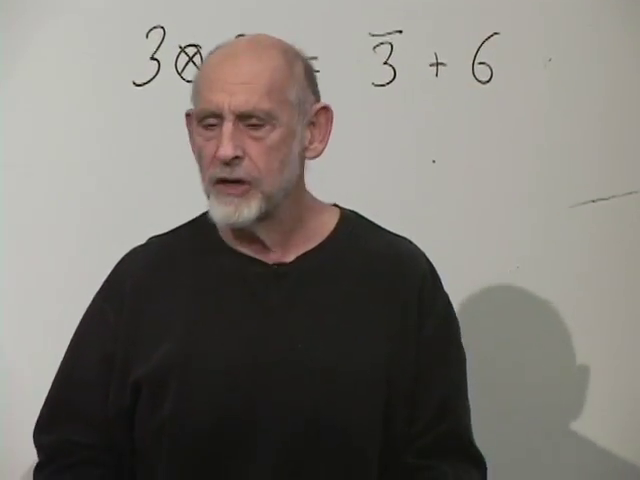
\includegraphics[width=0.68\textwidth]{lecture_04_figure_04.png}
\caption{Произведение двух кварков распадается на антитриплет и секстет.}
\lectureframe{00:39:33}
\end{figure}

Антитриплет можно явно представить, свёртывая два кварковых
индекса с инвариантным тензором эпсилон,
\begin{equation}
(qq)^k_{\bar 3}
=\frac{1}{\sqrt2}\epsilon^{kij}q_iq_j.
\end{equation}
Этот объект имеет 3 компоненты и преобразуется как антикварк. Шесть
симметричных комбинаций образуют секстет. Смысл не в том, что два кварка динамически
превращаются в антикварк; смысл в том, что один сектор их цветовой волновой
функции имеет тот же закон преобразования, что и антикварк.

\subsection{Кварк и антикварк: \texorpdfstring{\(\boldsymbol 3\otimes\bar{\boldsymbol 3}\)}{3 x анти-3}}

Цветовое состояние кварк--антикварк можно рассматривать как \(3\times3\)-матрицу
\(M_i{}^j=q_i\bar q^j\). Всякая такая матрица единственным образом разлагается на следовую и
бесследовую части,
\begin{equation}
M=\frac{\operatorname{tr}M}{3}\boldsymbol 1
+\left(M-\frac{\operatorname{tr}M}{3}\boldsymbol 1\right).
\end{equation}
След — это одна инвариантная компонента, а бесследовая часть имеет 8
компонент. Поэтому
\begin{equation}
\boldsymbol 3\otimes\bar{\boldsymbol 3}
=\boldsymbol 1\oplus\boldsymbol 8.
\label{eq:l4-three-times-threebar}
\end{equation}
С точностью до нормировки синглет имеет вид
\begin{equation}
\ket{1}_{q\bar q}
=\frac{1}{\sqrt3}
(\ket{r\bar r}+\ket{g\bar g}+\ket{b\bar b}).
\end{equation}
Он не может смешаться ни с чем другим, поскольку инвариантен. Остальные 8
линейных комбинаций перемешиваются между собой. Они реализуют присоединённое
представление, то самое представление, в котором преобразуются 8
генераторов.

\subsection{Три кварка}

Добавим третий кварк к разложению из уравнения~\eqref{eq:l4-three-times-three}. Ветвь
антитриплета даёт
\begin{equation}
\bar{\boldsymbol 3}\otimes\boldsymbol 3
=\boldsymbol 1\oplus\boldsymbol 8,
\end{equation}
так что произведение трёх кварков содержит синглет. Полностью имеем,
\begin{equation}
\boldsymbol 3\otimes\boldsymbol 3\otimes\boldsymbol 3
=\boldsymbol 1\oplus\boldsymbol 8\oplus\boldsymbol 8
\oplus\boldsymbol{10}.
\label{eq:l4-three-quark-full}
\end{equation}
Цветовой синглет — это полностью антисимметричная комбинация красный--зелёный--синий,
\begin{equation}
\ket{1}_{qqq}
=\frac{1}{\sqrt6}\epsilon^{ijk}\ket{q_iq_jq_k}.
\label{eq:l4-baryon-singlet}
\end{equation}
Поскольку \(\epsilon^{ijk}\) обращается в нуль всякий раз, когда два индекса совпадают, каждый
ненулевой член содержит один красный, один зелёный и один синий кварк, причём знаки
чередуются при перестановке.

\begin{classroomqa}
\audiencequestion{Разве несинглетные комбинации просто маловероятны, так что их вероятностями можно пренебречь?
\lecturetimestamp{00:46:02}}
\lecturerresponse{Нет. Дело в энергии, а не в малой вероятности. Изолированный несинглет протягивал бы цветовое поле на сколь угодно большие расстояния и в режиме конфайнмента требовал бы неограниченной энергии. Динамика, стоящая за этим утверждением, будет развита ниже.}
\end{classroomqa}

\subsection{Октет глюонов}

Глюонное поле преобразуется как октет в уравнении~\eqref{eq:l4-three-times-threebar}. По отношению к цвету оно несёт
один триплетный индекс и один антитриплетный индекс, причём синглетная следовая часть удалена.
Схематически,
\begin{equation}
q\sim\boldsymbol 3,
\qquad
\bar q\sim\bar{\boldsymbol 3},
\qquad
G\sim\boldsymbol 8.
\end{equation}
Эти символы обозначают законы преобразования; частицы не равны буквально
целым числам 3 и 8.

Девятая цветовая комбинация кварк--антикварк, пропорциональная единичной матрице,
является синглетом и не смешивается с октетом. Поэтому её опущение
математически непротиворечиво: калибровочное поле \(SU(3)\) бесследово и имеет 8
компонент, а не 9, как калибровочное поле \(U(3)\).

\begin{classroomqa}
\audiencequestion{Почему природа не включает дополнительный синглетный глюон?
\lecturetimestamp{00:49:00}}
\lecturerresponse{Непосредственный ответ теории групп таков: синглет образует отдельный инвариантный сектор, поэтому октет замкнут и без него. Более глубокая причина выбора \(SU(3)\), а не \(U(3)\), здесь не выводится; это часть калибровочной структуры, выведенной из феноменологии КХД.}
\end{classroomqa}

\section{Цветовые синглеты как адроны}

Свободные частицы сильного взаимодействия с конечной массой являются цветовыми синглетами.
Это не означает, что кварки или глюоны нереальны; это означает, что они не встречаются как
изолированные асимптотические частицы. Элементарные схемы построения синглетов таковы:
\begin{equation}
qqq,
\qquad
q\bar q,
\qquad
GG\ \text{and higher gluonic products}.
\end{equation}
Они приводят соответственно к барионам, мезонам и глюболам. Произведения нескольких
уже бесцветных объектов, разумеется, снова бесцветны, так что из этих ингредиентов можно построить
и более сложные многоадронные состояния.

\begin{classroomqa}
\audiencequestion{Как называются синглеты из трёх кварков и из кварка--антикварка, и могут ли глюоны тоже образовывать синглеты?
\lecturetimestamp{00:51:38}}
\lecturerresponse{Синглет из трёх кварков — это барион; синглет кварк--антикварк — мезон. Глюоны тоже могут объединяться в цветовые синглеты. Простейшие такие сильно взаимодействующие состояния называются глюболами, и в них могут участвовать более двух глюонов.}
\end{classroomqa}

Три кварка со спином 1/2 всегда объединяются в состояние с суммарным полуцелым спином, хотя орбитальный угловой момент может изменить, какое именно полуцелое значение реализуется. Мезоны кварк--антикварк имеют целый спин. Глюболы, состоящие только из глюонов, также имеют целый спин.

В случае двух глюонов первое утверждение на доске — это лишь подсчёт,
\begin{equation}
8\times8=1+63.
\end{equation}
Всего имеется 64 цветовых состояния; одна комбинация является синглетом, а остальные 63 принадлежат несинглетным секторам.

\begin{figure}[htbp]
\centering
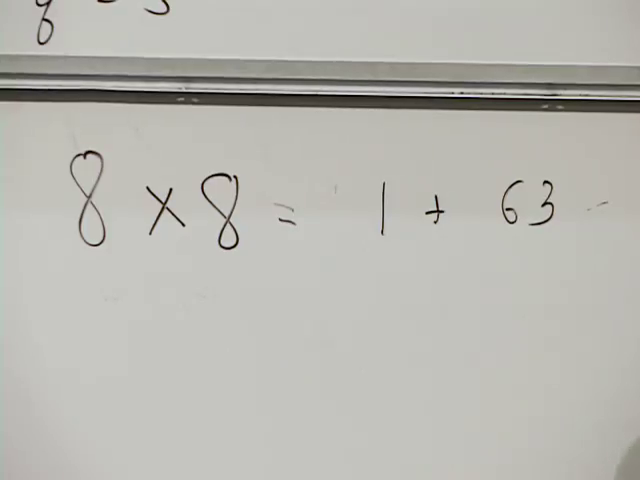
\includegraphics[width=0.68\textwidth]{lecture_04_figure_05.png}
\caption{Подсчёт числа состояний двух глюонов на доске: один синглет среди 64 состояний.}
\lectureframe{00:53:44}
\end{figure}

Полное разложение на неприводимые представления имеет вид
\begin{equation}
\boldsymbol 8\otimes\boldsymbol 8
=\boldsymbol 1\oplus\boldsymbol 8_S\oplus\boldsymbol 8_A
\oplus\boldsymbol{10}\oplus\overline{\boldsymbol{10}}
\oplus\boldsymbol{27}.
\label{eq:l4-eight-times-eight}
\end{equation}
Размерности складываются правильно:
\begin{equation}
1+8+8+10+10+27=64.
\end{equation}
Два октета — разные инвариантные подпространства: одно симметрично, другое антисимметрично при перестановке двух множителей в присоединённом представлении. Синглет — это двухглюонный цветовой канал, из которого можно построить состояние глюбола.
\editorialnote{На доске сначала дано только \(8\times8=1+63\). Более поздний обмен репликами в аудитории добавляет приведённые размерности неприводимых представлений; черты сверху и обозначения симметрии здесь восстановлены в стандартных обозначениях \(SU(3)\).}

\subsection{Почему наблюдаемые электрические заряды целочисленны}

Заряды кварков бывают двух типов,
\begin{equation}
Q_{\mathrm{up\text{-}like}}=+\frac23,
\qquad
Q_{\mathrm{down\text{-}like}}=-\frac13.
\end{equation}
Поэтому суммарный заряд трёх кварков является целым: \(-1,0,+1,\text{ or }+2\),
в зависимости от того, сколько из них относятся к up-типу. Пара кварк и антикварк аналогично имеет
заряд \(0\) или \(\pm1\). Глюоны не несут электрического заряда. Следовательно, базовые цветовые
синглеты, построенные из наблюдаемых кварковых представлений, имеют целочисленный электрический
заряд, хотя их составляющие несут дробный заряд.

\begin{classroomqa}
\audiencequestion{Каков электрический заряд странного кварка?
\lecturetimestamp{00:56:08}}
\lecturerresponse{Он относится к down-типу, поэтому его заряд равен \(-1/3\). Во всех трёх семействах повторяется одна и та же схема зарядов: \((u,d)\), \((c,s)\) и \((t,b)\), с зарядами \(+2/3\) и \(-1/3\) в каждой паре.}
\end{classroomqa}

Цветовая синглетность и целочисленность электрического заряда при таком наборе частиц тесно связаны, но это не тождественные математические утверждения. Целочисленность также опирается на только что записанные конкретные присвоения электрических зарядов в Стандартной модели.

\begin{classroomqa}
\audiencequestion{Является ли цветовой синглет запутанным состоянием, и имеет ли это тот же смысл, что и запутанная пара в эксперименте Белла?
\lecturetimestamp{00:56:58}}
\lecturerresponse{Синглетная цветовая волновая функция, безусловно, является запутанной: это когерентная суперпозиция, а не произведение отдельно определённых цветов. В принципе её составляющие можно разделить, но конфайнмент делает такое разделение всё более энергетически затратным и в конечном счёте порождает новые адроны. Поэтому это не удобная система для манипуляций в стиле эксперимента Белла, хотя само состояние запутано.}
\end{classroomqa}

\section{Что означают уравнения с тензорным произведением}

На этом этапе таблицы умножения заслуживают более конкретного объяснения.
Пусть \(\psi_i\) и \(\phi_j\) — операторы, создающие два объекта со спином 1/2; они могут описывать два вида частиц, например электрон и протон, либо две копии одного и того же вида, если учтена соответствующая статистика.
Каждый индекс принимает два значения. Четыре произведения
\begin{equation}
\psi_\uparrow\phi_\uparrow,
\quad
\psi_\uparrow\phi_\downarrow,
\quad
\psi_\downarrow\phi_\uparrow,
\quad
\psi_\downarrow\phi_\downarrow
\end{equation}
натягивают пространство тензорного произведения.

Если элемент группы действует как \(U\) на каждом сомножителе, то на
произведение он действует как \(U\otimes U\). В компонентах,
\begin{equation}
\psi_i\phi_j
\longmapsto
U_i{}^kU_j{}^\ell\psi_k\phi_\ell.
\label{eq:l4-product-action}
\end{equation}
Это четырёхмерное представление, но оно приводимо. Антисимметричная комбинация
\begin{equation}
\frac{1}{\sqrt2}
(\psi_\uparrow\phi_\downarrow
-\psi_\downarrow\phi_\uparrow)
\end{equation}
переходит в себя, тогда как три симметричные комбинации переходят друг в друга. В базисе, согласованном с этими комбинациями, каждая матрица
представления на произведении имеет блочно-диагональный вид,
\begin{equation}
D_{2\otimes2}(g)
\sim
\begin{pmatrix}
1&0\\
0&D_3(g)
\end{pmatrix}.
\label{eq:l4-spin-block-diagonal}
\end{equation}

\begin{classroomqa}
\audiencequestion{Какая операция представлена уравнением вида \(\boldsymbol 3\otimes\boldsymbol 3=\bar{\boldsymbol 3}\oplus\boldsymbol 6\)?
\lecturetimestamp{00:57:51}}
\lecturerresponse{Левая часть задаёт пространство составных состояний. Группа действует на оба сомножителя и потому перемешивает базисные состояния произведения. Правая часть говорит, что смена базиса разделяет эти состояния на инвариантные наборы: 3 антисимметричные комбинации, преобразующиеся как антитриплет, и 6 симметричных комбинаций, преобразующихся как секстет. Знак плюс означает прямую сумму альтернатив, а не обычное численное сложение.}
\end{classroomqa}

\begin{classroomqa}
\audiencequestion{Откуда мы знаем, что 9 состояний распадаются как \(3+6\) или \(1+8\), а не, скажем, как \(2+7\)?
\lecturetimestamp{01:04:39}}
\lecturerresponse{Одного лишь подсчёта размерностей недостаточно, чтобы определить разбиение. Нужно знать, какими неприводимыми представлениями обладает \(SU(3)\), и построить инвариантные подпространства, например симметризуя индексы, антисимметризуя их или отделяя следовую часть от бесследовой. Полная классификация требует большей теории групп; здесь мы используем только представления, нужные для кварков и глюонов.}
\end{classroomqa}

Инвариантный тензор эпсилон делает построение синглета наглядным. Для
\(SU(2)\),
\begin{equation}
\epsilon_{ij}U^i{}_kU^j{}_\ell
=(\det U)\epsilon_{k\ell}
=\epsilon_{k\ell}.
\end{equation}
Следовательно, \(\epsilon_{ij}\psi^i\phi^j\) инвариантно. Для \(SU(3)\)
трёхиндексная версия даёт
\begin{equation}
\epsilon_{ijk}U^i{}_aU^j{}_bU^k{}_c
=(\det U)\epsilon_{abc}
=\epsilon_{abc},
\end{equation}
что доказывает инвариантность трёхкваркового состояния в
уравнении~\eqref{eq:l4-baryon-singlet}.

\begin{classroomqa}
\audiencequestion{Можно ли явно показать, почему синглет не преобразуется?
\lecturetimestamp{01:07:18}}
\lecturerresponse{Да. Сверните все фундаментальные индексы с полностью антисимметричным тензором эпсилон. При преобразовании произведение матриц умножает эпсилон на \(\det U\). Для специальной унитарной матрицы этот определитель равен единице, так что свёрнутое состояние не изменяется. В \(SU(2)\) это доказывает синглет двух спинов; в \(SU(3)\) — красный--зелёный--синий трёхкварковый синглет.}
\end{classroomqa}

\begin{classroomqa}
\audiencequestion{Каково полное разложение двух глюонных октетов?
\lecturetimestamp{01:09:24}}
\lecturerresponse{Это разложение из уравнения~\eqref{eq:l4-eight-times-eight}: один синглет, два октета, декуплет, антидекуплет и 27-мерное представление. Существует ровно одна цветовая синглетная комбинация двух октетных индексов.}
\end{classroomqa}

\begin{classroomqa}
\audiencequestion{Каково соответствующее полное разложение для трёх кварков?
\lecturetimestamp{01:11:51}}
\lecturerresponse{Физически существенный ответ состоит в том, что оно содержит один синглет. Полное вычисление даёт уравнение~\eqref{eq:l4-three-quark-full}: один синглет, два октета и один декуплет, всего \(1+8+8+10=27\) состояний.\editorialnote{Во время этого обмена репликами лектор не вспоминает полного разложения \(3\otimes3\otimes3\). Стандартное дополнение приведено здесь явно и помечено как редакторское, а не приписано устному ответу.}}
\end{classroomqa}

Та же идея распространяется и на пространство двух глюонов. В наивном базисе тензорного произведения
\(SU(3)\) действует посредством матриц \(64\times64\). В базисе, согласованном с
неприводимыми компонентами, эти матрицы блочно-диагональны,
\begin{equation}
\begin{aligned}
D_{8\otimes8}(g)
&\sim
\operatorname{diag}\bigl(
1,D_{8_S}(g),D_{8_A}(g),
\\
&\hspace{4.8em}
D_{10}(g),D_{\overline{10}}(g),D_{27}(g)
\bigr).
\end{aligned}
\end{equation}
Ни один блок не смешивается с другим, хотя состояния внутри каждого блока смешиваются между
собой.

\begin{classroomqa}
\audiencequestion{Является ли разложение тензорного произведения просто переходом к базису, в котором большая матрица представления становится блочно-диагональной?
\lecturetimestamp{01:12:02}}
\lecturerresponse{Именно так. Для двух спинов четырёхмерная матрица превращается в одномерный синглетный блок и трёхмерный триплетный блок. Для двух глюонов 64-мерная матрица превращается в блоки размерностей \(1,8,8,10,10,\text{ and }27\). Каждый блок замкнут относительно любого группового преобразования.}
\end{classroomqa}

\begin{classroomqa}
\audiencequestion{Есть ли название у одной из таких замкнутых частей внутри полного пространства тензорного произведения?
\lecturetimestamp{01:14:55}}
\lecturerresponse{Это инвариантное подпространство, несущее подпредставление. Если его нельзя разложить дальше, оно несёт неприводимое представление, или ирреп. Полное тензорное произведение есть прямая сумма этих неприводимых компонент.\editorialnote{В источнике искомый термин в аудитории так и не произносится. В ответе приведена стандартная терминология теории представлений.}}
\end{classroomqa}

\begin{classroomqa}
\audiencequestion{Когда несинглетные десятиплеты и другие представления называют несуществующими, означает ли это, что ими следует полностью пренебречь?
\lecturetimestamp{01:15:36}}
\lecturerresponse{Они являются законными цветовыми секторами и важны в промежуточных вычислениях, но не появляются в лаборатории как изолированные частицы конечной энергии. Конфайнмент, а не какой-либо изъян теории представлений, не даёт им стать свободными асимптотическими состояниями.}
\end{classroomqa}

\section{От идеи цвета Намбу к конфайнменту}

Идея цвета возникла раньше окончательной формулировки КХД. Ёитиро Намбу уже
в начале 1960-х годов понял, что скрытое квантовое число, принимающее три значения, могло
решить поразительную проблему: кварки несут дробный электрический заряд, однако свободных
частиц с дробным зарядом не наблюдается. Если физические состояния вынуждены
быть цветовыми синглетами, кварки встречаются в описанных выше комбинациях с
целым зарядом. Оставшийся вопрос — динамический: что вынуждает все свободные
состояния конечной энергии быть синглетами?

Начнём с электромагнитной аналогии. Заряд и противоположный ему заряд притягиваются. Если сближать их, энергия уменьшается; чтобы сблизить одноимённые заряды, нужно совершить работу. Само поле запасает положительную энергию,
\begin{equation}
E_{\mathrm{field}}
=\frac12\int d^3x\,\boldsymbol E^2
\end{equation}
в простых электростатических единицах. При ненулевом суммарном заряде поле простирается далеко за пределы системы, тогда как у тесно связанной нейтральной пары есть лишь короткодействующее дипольное поле. Поэтому нейтрализация убирает энергию поля из внешней области.

Представим, что электромагнитное взаимодействие стало чрезвычайно сильным. Энергетическая цена поля за ненулевой суммарный заряд стала бы настолько большой, что низкоэнергетические объекты в подавляющем большинстве были бы нейтральными, а извлечение заряженной составной части могло бы стать непомерно дорогим. Nambu перенёс эту интуицию на цвет: восемь цветовых зарядов являются источниками восьми глюонных полей, так что большая энергия цветового поля могла бы запретить существование изолированных несинглетов.

Эта интуиция по существу верна, но в QCD есть решающая новая особенность. Фотон не несёт электрического заряда, тогда как глюон несёт цвет. Фотон не является источником классического электромагнитного поля, а уравнения Максвелла линейны: две электромагнитные волны складываются по принципу суперпозиции и проходят друг сквозь друга. Глюон преобразуется по октетному представлению цвета, поэтому глюоны являются источниками других глюонов и взаимодействуют с ними. Даже разные части одного и того же глюонного поля взаимодействуют. Следовательно, неабелево калибровочное поле нелинейно.

\subsection{Трубки потока и линейный потенциал}

На больших расстояниях самодействие глюонов не позволяет цветовому потоку расплываться, как обычное электрическое дипольное поле. Поток сжимается в трубку, соединяющую кварк с антикварком. Напряжённость поля и площадь поперечного сечения длинной трубки приблизительно постоянны, поэтому в ней запасается приблизительно постоянная энергия на единицу длины. Если \(\sigma\) обозначает это натяжение струны, то
\begin{equation}
V(R)\simeq\sigma R+\text{constant}
\qquad (R\ \text{large}).
\label{eq:l4-linear-potential}
\end{equation}

\begin{figure}[htbp]
\centering
\includegraphics[width=0.78\textwidth]{lecture_04_figure_06.png}
\caption{Цветовой поток собран в длинную трубку между кварком и антикварком.}
\lectureframe{01:31:35}
\end{figure}

Такой потенциал сильнее кулоновского, модуль которого убывает как \(1/R\).
Если раздвигать цветовые источники дальше, сила не убывает неограниченно; трубка удлиняется, и энергия продолжает расти. Одинокий цветовой заряд в бесконечном объёме потребовал бы трубку, тянущуюся без конца, и, следовательно, неограниченную энергию. В этом и состоит практический смысл утверждения, что только цветовые синглеты имеют асимптотические состояния с конечной энергией.
\editorialnote{Обозначение натяжения струны и явный вид потенциала на больших расстояниях количественно выражают утверждение источника о том, что однородная трубка потока несёт однородную энергию на единицу длины.}

\subsection{Разрыв струны и джеты}

Предположим, что жёсткое столкновение приходится на один из кварков внутри мезона. Кварк начинает удаляться, но позади него растягивается трубка потока. Он может потерять свою кинетическую энергию, и его втянут обратно. Однако чаще, как только запасённая энергия поля становится достаточно большой, вакуум рождает новую пару кварк--антикварк. Новый антикварк служит концом потока, связанного с уходящим кварком, а новый кварк — концом потока, связанного с исходным антикварком. Один растянутый синглет превращается в два более коротких синглета,
\begin{equation}
(q\bar q)_{\mathrm{stretched}}
\longrightarrow
(q\bar q)+(q\bar q).
\label{eq:l4-string-breaking}
\end{equation}

\begin{figure}[htbp]
\centering
\includegraphics[width=0.78\textwidth]{lecture_04_figure_07.png}
\caption{Рождение пары разрывает одну растянутую трубку потока на две цветосинглетные трубки.}
\lectureframe{01:34:52}
\end{figure}

\begin{classroomqa}
\audiencequestion{Если выбитый кварк имеет достаточно энергии, чтобы продолжать растягивать трубку, что ещё может произойти, кроме того, что его втянут обратно?
\lecturetimestamp{01:33:50}}
\lecturerresponse{Трубка может разорваться за счёт рождения пары кварк--антикварк. Её энергия превращается в массу и кинетическую энергию новой пары. Концы пересоединяются в два синглета, так что процесс порождает дополнительные мезоны, а не изолированный кварк.}
\end{classroomqa}

Если один из этих партонов всё ещё несёт большой импульс, процесс повторяется. Результатом становится каскад цветосинглетных адронов, коллимированный вокруг исходного направления партона: джет. Это превращение энергичных кварков и глюонов в адроны называется адронизацией. Об инициирующем цветном объекте судят по джету; сам по себе он никогда не наблюдается.

\begin{classroomqa}
\audiencequestion{При разрыве струны образуются только мезоны или в джете могут появляться и другие адроны?
\lecturetimestamp{01:35:20}}
\lecturerresponse{Конечно, могут появляться и другие адроны. Единственное цветовое требование состоит в том, чтобы конечные наблюдаемые объекты были синглетами. Мезоны — самый простой вариант для одного разрыва, но могут также рождаться барионы, антибарионы и более сложные синглетные комбинации.}
\end{classroomqa}

Три кварка могут замыкать свои потоки в цветосинглетном узле. Трёхветвенная картина является динамическим аналогом антисимметричного эпсилон-тензора в уравнении~\eqref{eq:l4-baryon-singlet}: из полного бариона не выходит никакого суммарного цветового потока.

\begin{figure}[htbp]
\centering
\includegraphics[width=0.72\textwidth]{lecture_04_figure_08.png}
\caption{Трёхветвевой узел цветового потока для бариона, под схемой разрыва мезонной струны.}
\lectureframe{01:36:12}
\end{figure}

\section{Калибровочные поля, сохраняющиеся заряды и стандартная модель}

На данном уровне калибровочную теорию можно понимать как теорию, в которой сохраняющийся заряд является источником фотоноподобного поля. Электрический заряд является источником электромагнитного поля; восемь цветовых зарядов являются источниками восьми глюонных полей. Более глубокая формулировка делает симметрию локальной и вводит связность, которая сравнивает внутренние состояния в соседних точках пространства-времени, но для развиваемой здесь картины конфайнмента эта конструкция не нужна.
\editorialnote{Формулировка через локальную симметрию — это тот стандартный, более глубокий смысл калибровочной теории, на который источник ссылается, но который сознательно откладывает.}

Симметрия, сохраняющийся заряд и поток тесно связаны. Если силовые линии поля могут оканчиваться только на зарядах, то источник не может просто исчезнуть, оставив свой поток оборванным. Не может и всё его удалённое поле исчезнуть мгновенно, потому что изменения поля распространяются причинно. В локальной форме та же физика выражается уравнением непрерывности,
\begin{equation}
\frac{\partial\rho}{\partial t}
+\boldsymbol\nabla\cdot\boldsymbol j=0,
\end{equation}
которое говорит, что заряд может покинуть область, только перетекая через её границу. Аргумент через силовые линии — это геометрическая картина этого локального закона сохранения.

Теперь мы можем поместить результат в рамки стандартной модели. Цвет даёт восемь генераторов \(SU(3)\) и соответствующие им восемь глюонных полей. Абелев сектор даёт один генератор и одно калибровочное поле. Ещё три генератора принадлежат дополнительной группе \(SU(2)\), а не обычному пространственному угловому моменту. До нарушения симметрии калибровочная структура имеет вид
\begin{equation}
SU(3)_c\times SU(2)_L\times U(1)_Y,
\end{equation}
с \(8+3+1=12\) генераторами. Следующая задача — понять электрослабую группу \(SU(2)\), затем поле Хиггса и то, как возникают наблюдаемые фотон, \(W^\pm\) и \(Z\).
\editorialnote{Источник считает фотон вместе с восемью глюонами и описывает оставшийся множитель как \(SU(2)\times U(1)\). В ненарушенной стандартной модели абелевым множителем является гиперзаряд \(U(1)_Y\); фотон появляется только после электрослабого смешивания.}

Теперь центральная цепочка завершена. Абстрактные группы действуют через представления; бесконечно малые генераторы являются сохраняющимися зарядами; кварки, антикварки и глюоны реализуются в \(\boldsymbol 3\), \(\bar{\boldsymbol 3}\) и \(\boldsymbol 8\); тензорные произведения выделяют адроны-синглеты; а нелинейное глюонное поле превращает отбор синглетов в физическое явление конфайнмента.